\documentclass[smallextended]{svjour3}
%\usepackage{cite}
% *** GRAPHICS RELATED PACKAGES ***
%
  \usepackage[pdftex]{graphicx}
%
\usepackage[cmex10]{amsmath}


% *** ALIGNMENT PACKAGES ***
%
\usepackage{array}
%\usepackage{fixltx2e}

\usepackage{stfloats}
% LaTeX2e). It also provides a command:
\fnbelowfloat

\usepackage{booktabs}
\usepackage{amssymb}
\usepackage{amsmath}
\usepackage{pgf}
\usepackage{tikz}
\usetikzlibrary{arrows,positioning}
\usepackage[hyphens]{url}
\usepackage{color}
\usepackage{graphicx}
\usepackage{xspace}
\newcommand*{\eg}{e.g.\@\xspace}
\newcommand*{\ie}{i.e.\@\xspace}
\newcommand*{\vs}{vs.\@\xspace}

\newcommand*{\EMD}{\mathrm{EMD}}

% correct bad hyphenation here
\hyphenation{wave-let}

\usepackage{color}
\newcommand{\vl}[1]{\textcolor{orange}{Vincent : #1}}
\newcommand{\gl}[1]{\textcolor{red}{Gr\'egoire : #1}}
\newcommand{\ja}[1]{\textcolor{magenta}{Joakim : #1}}
\newcommand{\ml}[1]{\textcolor{blue}{ Mathieu : #1}}

\usepackage[backend=bibtex,style=numeric-comp,sorting=none,firstinits=true]{biblatex}
\bibliography{biblio}
%\renewcommand{\baselinestretch}{2}


\begin{document}
%
% paper title
% can use linebreaks \\ within to get better formatting as desired
% Do not put math or special symbols in the title.
%\title{An evaluation framework for event detection using a morphological model of acoustic scenes}
\title{Relevance-based Quantization of Scattering Features for Unsupervised Mining of Environmental Audio}
\titlerunning{Relevance-based Quantization of Scattering Features}

\author{Vincent Lostanlen\thanks{This work is supported by the ERC InvariantClass grant 320959.}, Gr\'egoire Lafay, Joakim And\'en, and Mathieu Lagrange}


% make the title area
\maketitle

% As a general rule, do not put math, special symbols or citations
% in the abstract or keywords.
\begin{abstract}
The emerging field of computational ecoacoustics aims at retrieving high-level information from acoustic scenes recorded by some network of sensors. These networks gather large amounts of data requiring analysis. To decide which parts to inspect manually, we need tools that automatically mine the data, identifying recurring patterns and isolated events. This requires a similarity measure for acoustic scenes that does not impose strong assumptions on the data.

The state of the art in audio similarity measurement is the ``bag-of-frames'' approach, which models a recording using summary statistics of short-term audio descriptors, such as mel-frequency cepstral coefficients (MFCCs). They successfully characterize static scenes with little variability in auditory content, but cannot accurately capture scenes with a few salient events superimposed over static background.
To overcome this issue, we propose a two-scale representation which describes a recording using clusters of scattering coefficients. The scattering coefficients capture short-scale structure, while the cluster model captures longer time scales, allowing for more accurate characterization of sparse events. Evaluation within the acoustic scene similarity framework demonstrates the superiority of the proposed approach.
\keywords{
unsupervised learning \and data mining \and acoustic signal processing \and wavelet transforms \and audio databases \and content-based retrieval \and nearest neighbor searches \and acoustic sensors \and environmental sensors.}
% \PACS{PACS code1 \and PACS code2 \and more}
\end{abstract}


\section{Introduction}

The amount of audio data recorded from our sonic environment has grown considerably over the past decades.
In order to measure the effect of human activity and climate change on animal biodiversity, researchers have recently undertaken a massive deployment of acoustic sensors throughout the world \cite{warren2006urban, NessSST13, stowell13b}.
In addition, recent work has explored acoustic monitoring for characterization of human pleasantness in urban areas \cite{guyot2005urban, ricciardi2015sound}, as well as the prediction of annoyance due to traffic \cite{gloaguen}.
Since they bear a strong societal impact and raise many scientific challenges, we believe that these applications are of considerable interest for the signal processing community.

This work falls in the realm of ecoacoustics, an emerging field in computational bioacoustics, which is the interdisciplinary study of relationships between natural or anthropogenic sounds and their environments at the intersection of ecology, acoustics and computer science \cite{krause}. %Despite identified needs, the field of signal-based ecoacoustics is still in its infancy.
%Consequently, few well-designed datasets are readily available for evaluation purposes.
An important problem in this field is that manually analysing the recorded data to identify the quantities of interest is very costly \cite{wimmer2013sampling}. Some sort of pre-screening is therefore needed to reduce the need for human expert listening and annotation.

The most straightforward approach is to assume a closed set of events of interests like sounds of animals expected to live near the acoustic sensors, train models for them and perform automatic annotation \cite{}. A given time interval, for example a single day, is then represented by the number of events within the predefined typology that have been detected in that period of time. This approach allows the scientist to drastically reduce the amount of information that needs to be processed. However, this approach has two drawbacks. The first is the reliance to trained models whose behavior on unseen data (such as different sensors) is prone to errors and cannot be always be trusted. More importantly, it is based on \textit{a priori} knowledge and thus cannot be considered for exploratory analysis where the quantities of interest have yet to be defined.

In order to identify which parts needs human inspection, one needs tools that can mine data and annotate to whether recurring patterns  or sparsely distributed events to study anomalous or scarce behaviors. The latter allowing the scientist to then annotate only a representative audio of the periods of time with recurring patterns and the former to potentially discover unforseen phenomena.

With this aim, one needs to design an algorithm to perform an acoustic similarity retrieval, where the audio fragments judged ``most similar'' to a given query section are extracted from some larger dataset. This requires the audio fragments to be represented in some way that captures their distinctive qualities. This has been achieved by bag-of-frames approaches \cite{aucouturier2007bag}, which attempt to describe the auditory scene recording using summary statistics. Unfortunately, since this only captures the average structure of the scene, the approach often fails when presented with scenes which are dynamic and contain episodic, distinct sound events that discriminate the scene from others. Indeed, experiments in cognitive psychology \cite{dubois2006cognitive} and cognitive neurosciences \cite{nelken2004processing} suggest that this matches more closely human acoustic perception of acoustic scenes. We believe that the failure to model such distinct events is one of the reason why this approach is found to be insufficient when considering evaluation datasets of typical sizes \cite{lagrange:hal-01082501}.

%To design better representations for the similarity retrieval task, we draw inspiration from a closely related, and more mature, field of investigation: the classification of acoustic scenes. This task, consisting of predicting scene labels from audio recordings, is narrower in its range of applications, but has the advantage of being rooted in the cognitive psychology of categorization \cite{dubois2006cognitive,guastavino_ideal_2006}. In addition, it has received significant attention from the data mining community for some time, resulting in the availability of well-designed datasets and competitive algorithms for solving it.

Addressing this task first requires the ability to capture meaningful aspects within the signal at small time-scales.
In other words, how do we represent an extract of the auditory scene signal over a sub-second interval?
A standard tool for this are the mel-frequency cepstral coefficients (MFCCs), originally developed for speech processing \cite{davis-mermelstein}, but which have found wider use in recent years in music information retrieval \cite{logan} and environmental audio processing \cite{aucouturier2007bag}.
A richer set of features is found in the scattering transform, a generic signal representation which has enjoyed significant success in various audio classification tasks \cite{Anden2014,chudacek}.
This is because the scattering transform cascades wavelet convolutions and pointwise nonlinearities, thus imitating the architecture of a convolutional neural network \cite{lee,lostanlen-deep-spiral,soundnet,arandjelovic-zisserman}.

For the task at at hand, scattering features have the advantage of not requiring training and thus potentially lead to wider range of application than trained features. Indeed, the task at hand is the mining of yet unheard audio datasets and the properties of the audio that are of interest remains to be defined, thus leading to an unserpervised setting.


%The next question is the choice of a classifier. Here, a class of particularly successful algorithms train a classifier, such as a support vector machine (SVM) \cite{cristianini2000introduction}, to discriminate between short extracts of an auditory scene, and at the classification stage divide the signal into short extracts which are classified separately before pooling the classification results to reach a final decision. This last step is known as late integration and is crucial to the success of these methods, since it allows the classifier to concentrate on the short, distinct sound events that discriminate between scenes. The success of the late integration technique again leads credence to the idea that rare, distinct events in an auditory scene are sufficient to characterize it almost completely. Combining scattering transforms for low-level representation with late-integrated SVMs for classifying the scene at a higher level, we obtain a competitive auditory scene classification system, demonstrating the usefulness of both concepts for this task.

%we can emulate their selection behavior by quantizing the auditory scene and defining a distance over this quantization.
We also propose a new model for acoustic scenes, where the signal is represented at sub-second scales by scattering transforms, while larger scales are captured by an unsupervised method that quantizes the scattering coefficients into a given number of clusters. We then use these clusters to define a set of distances that can subsequently be used for similarity retrieval. \vl{The verb use is repeated in the previous sentence.} Testing this approach on a scene retrieval task, we obtain significant improvements over traditional bag-of-frames and summary statistics models applied both to MFCCs and scattering coefficients.

Motivations of the proposed approach and a brief review of the state of the art in acoustic scene modeling are given in Section \ref{sec:soa}. We describe the scattering transform in Section \ref{sec:scattering}, discuss feature post-processing in Section \ref{sec:design} and propose a cluster-based scene description in Section \ref{sec:object}. Section \ref{sec:experiments} describes several experiments for the acoustic scene similarity retrieval task. Results are subsequently reported in Section \ref{sec:results}.

\section{Background} \label{sec:soa}

%One avenue of ecoacoustics research, originating in bioacoustics, attempts to identify species properties of vocalizations, for example to link animal vocalization with behavior\cite{au2008principles, stowell2014large}.

Computational bioacoustics usually refers to the numerical investigation of sound production, dispersion and reception in animals (including humans). A recent paradigm  processes the audio stream in a holistic way over large time-scales, without assuming that a single species is present throughout the recording. Automated systems belonging to this paradigm attempt to infer global properties of bioacoustic scenes, including biodiversity indices \cite{Bardeli2010}, migration patterns \cite{Obrist2010}, as well as marking time intervals of particular interest for detailed human inspection \cite{rosenstock2002landbird}.

%The same division is found in the field of auditory scene analysis, wherein the interest may either be 1) to isolate and identify precise events, \ie acoustic event detection (AED), or 2) to predict global attributes assigned to large time spans of audio, \ie acoustic scene classification (ASC).
In the closely related field of urban sound environment analysis, a popular approach is the bag of frames (BOF) introduced in this context by Aucouturier et al. \cite{aucouturier2007bag}, where a scene is modeled by high-level summary statistics computed from local features.
Recently, the proposed implementation using Gaussian mixture models (GMMs) of mel-frequency cepstral coefficients (MFCCs) has been demonstrated to perform comparably to a direct averaging of the features for a variety of tasks \cite{lagrange:hal-01082501}.
This contrasts with the typical morphology of acoustic scenes, which we believe is a ``skeleton of events on a bed of textures'' \cite{nelken2013} where a few discrete sound events are superimposed upon a stationary acoustic background.
As those distinct and sparse events are often highly relevant for the task at hand, it is arguably more beneficial to focus on characterizing these distinct events through describing the large-scale temporal evolution of auditory scenes rather than on summary statistics of short-term features.

This statement has some support in auditory psychology as well as sound synthesis based on summary statistics \cite{mcdermott2013summary}. For example, studies in the cognitive psychology of urban sound environments have shown that global sound level (perceived or measured) is not sufficient to fully characterize an acoustic scene \cite{guyot2005urban,kang2006urban}. Rather, it seems that cognitive processes such as sound environment quality perception \cite{dubois2006cognitive} or loudness judgment \cite{kuwano_memory_2003} rely upon higher-level cognitive attributes such as the identities of sound sources which compose the scene. It has been shown that, if available, the complete description of the scene in terms of event occurrences is powerful enough to reliably predict high-level cognitive classes. For example, the presence of birds is very likely to be heard in parks in urban areas and so are strong pleasantness indicators. Consequently, research in sound perception is now strongly focused on the contribution of specific sound sources in the assessment of sound environments \cite{ricciardi2015sound,lavandier2006contribution}. Although the complete set of events occurring within a given auditory stream may not be discernable even to human expects, research has shown that a small set of events (so-called markers) suffice to reliably predict many high-level attributes.

From a cognitive psychology perspective, the consensus is therefore that only a few distinct events are sufficient to describe an auditory scene, in contrast to BOF approaches which treat each observation the same and do not incorporate temporal structure between features. A method that takes this knowledge into account could therefore have potential for great impact in the modeling of acoustic scenes, provided that the representation of the representation of those distinct events is rich enough.

%Aside from \cite{aucouturier2007bag} and \cite{lagrange:hal-01082501} that consider the task of acoustic scene similarity retrieval, much of the work dedicated to acoustic scene modeling is applied to the classification task.
%An overview of the efforts for the latter task is provided by the IEEE Audio and Acoustic Signal Processing (AASP) Detection and Classification of Acoustic Scenes and Events (DCASE) challenge \cite{barchiesi2015acoustic}, held in 2013 to compare different approaches to scene classification.

%The methods that performed the best all follow a similar structure, where low-level feature representations, such as MFCCs, are calculated over short windows and fed separately to a classifier, such as a support vector machine (SVM) \cite{cortes-vapnik,cristianini2000introduction}, for training. During the classification stage, a given recording is similarly processed into short windows represented by feature vectors which are classified individually by the classifier. The individial class assignments are then combined through a majority vote which assigns a class to the whole recording. This last step is known as late integration and allows the classifier to work on individual, shorter-scale sound events instead of trying to classify the recording as a whole. By doing this, the classifier is able to identify and exploit the distinct events that characterize the scene instead of trying to model its average structure. This is in agreement with the psychoacoustic results related to the perception of auditory scenes presented above.


%\ml{These two last paragraphs are a bit out of place here, since we don't do classification in the paper. Perhaps there is some way to cut them down a bit?}

%\gl{Othe this r paper:} \cite{jiang2005svm, kalinli2009saliency, su2011environmental, ye2015acoustic, bisot2015hog, chakrabarty2015exploring, xue2015auditory}

%\subsection{Datasets}

 % The latter is also considered in this paper as a validation of the proposed approach. \ja{What does this last sentence mean?}

%In this paper, we shall demonstrate that the use of features based on the wavelet scattering transform together with object-based representation of the acoustic scene allows us to achieve state-of-the-art \ja{?} performance in both the ASSR and ASC paradigms.

\section{Wavelet scattering \label{sec:scattering}}

Scattering transforms are time-shift invariant representations of audio signals computed by applying auditory and modulation wavelet filter banks alternated with complex modulus nonlinearities.
This section first explains the importance of local invariance to time-shifting and stability to time-warping in the representation of acoustic scenes, then describes how the scattering transform is designed to satisfy these properties while retaining high discriminative power.

\subsection{Invariance and stability in audio signals}
The notion of invariance to time-shifting plays an essential role in acoustic scene similarity retrieval as well as acoustic scene classification.
Indeed, recordings may be shifted locally without affecting their similarity to other recordings.
To discard this superfluous source of variability, signals are first mapped into a time-shifting invariant feature space. These features are then used to calculate similarities or to train a classifier. Since invariance is ensured by the features, it does not have to be learned during this last model construction step.

Formally, given a signal $\boldsymbol{x}(t)$, we would like its translation $\boldsymbol{x_c}(t) = \boldsymbol{x}(t-c)$ to be mapped to the same feature vector provided that $|c| \ll T$ for some maximum duration $T$ that specifies the extent of the time-shifting invariance. We can also define more complicated transformations by letting $c$ vary with $t$. In this case, we have $\boldsymbol{x_\tau}(t) = \boldsymbol{x}(t-\tau(t))$ for some function $\tau$, which performs a time-warping of $\boldsymbol{x}(t)$ to obtain $\boldsymbol{x_\tau}(t)$. Time-warpings model various changes, such as small variations in pitch, reverberation, and rhythmic organization of events. These make up an important part of intra-class variability among natural sounds, so it is important for representation to be robust to such transformations.

The wavelet scattering transform, described below, has both of these desired properties: invariance to time-shifting and stability to time-warping. The stability condition can be formulated as a Lipschitz continuity property, which guarantees that the feature transforms of $\boldsymbol{x}(t)$ and $\boldsymbol{x_\tau}(t)$ are close together if $|\tau'(t)|$ is bounded by a small constant.

\subsection{Wavelet scalogram}
Our convention for the Fourier transform of a continuous-time signal $\boldsymbol{x}(t)$ is $\boldsymbol{\hat{x}}(\omega) = \int_{-\infty}^{+\infty} x(t) \exp(- \mathrm{i} 2\pi \omega t) \; \mathrm{d}t$.
Let $\boldsymbol{\psi}(t)$ a complex-valued analytic bandpass filter of
center frequency $\xi_1$ and bandwidth $\xi_1/Q_1$, where $Q_1$ is the quality factor of the filter.
A filter bank of wavelets is built by dilating $\boldsymbol{\psi}(t)$
according to a geometric sequence of scales $2^{\gamma_1/Q_1}$, obtaining
\begin{equation}
\boldsymbol{\psi_{\gamma_1}}(t) = 2^{-\gamma_1/Q_1} \boldsymbol{\psi}(2^{-\gamma_1/Q_1} t)\mbox{.}
\end{equation}
The variable $\gamma_1$ is a scale (an inverse log-frequency) taking integer values between $0$ and $(J_1 Q_1 - 1)$, where $J_1$ is the number of octaves spanned by the filter bank.
For each $\gamma_1$, the wavelet $\boldsymbol{\psi_{\gamma_1}}(t)$
has a center frequency of $2^{-\gamma_1/Q_1}\xi_1$ and a bandwidth of $2^{-\gamma_1/Q_1}\xi_1/Q_1$ resulting in the same quality factor $Q_1$ as $\boldsymbol{\psi}$.
In the following, we set $\xi_1$ to $20~\mathrm{kHz}$, $J_1$ to $10$, and the quality factor $Q_1$, which is also the number of wavelets per octave, to $8$. This results in the wavelet filters covering the whole range of human hearing, from $20~\mathrm{Hz}$ to $20~\mathrm{kHz}$. Setting $Q_1 = 8$ results in filters whose bandwidth approximates an equivalent rectangular bandwidth (ERB) scale \cite{Fastl2007}.

The wavelet transform of an audio signal
$\boldsymbol{x}(t)$ is obtained by convolution with all wavelet filters.
Applying pointwise complex modulus the transform yields
the wavelet scalogram
\begin{equation}
\boldsymbol{x_1}(t, \gamma_1)
= \vert \boldsymbol{x} \ast \boldsymbol{\psi_{\gamma_1}} \vert (t)\mbox{.}
\end{equation}
The scalogram bears resemblance to the constant-Q transform (CQT),
which is derived from the short-term Fourier transform (STFT) by averaging the frequency
axis into constant-Q subbands of center frequencies $2^{-\gamma_1/Q_1}\xi_1$.
Indeed, both time-frequency representations are indexed by time $t$ and log-frequency $\gamma_1$.
However, contrary to the CQT, the scalogram reaches a better time-frequency localization across the whole
frequency range, whereas the temporal resolution of the traditional CQT is fixed by the support of the STFT analyzing window. %\cite{Brown1992}
Therefore, the scalogram has a better temporal localization at high
frequencies than the CQT, at the expense of a greater computational cost
since the inverse fast Fourier transform routine must be called for each wavelet $\boldsymbol{\psi_{\gamma_1}}$ in the filter bank.
However, this allows us to observe amplitude modulations at fine temporal scales in the scalogram, down to $2Q_1/\xi_1$ for $\gamma_1 = 0$, of the order of $1\,\textrm{ms}$ given the aforementioned values of $Q_1$ and $\xi_1$.

To obtain the desired invariance and stability properties, the scalogram is averaged in time using a lowpass filter $\phi(t)$ with cut-off frequency $1/T$ (and approximate duration $T$), to get
\begin{equation}
\mathbf{S_1}\boldsymbol{x}(t, \gamma_1) = \boldsymbol{x_1}(\cdot, \gamma_1) \ast \phi(t),
\end{equation}
which is known as the set of first-order scattering coefficients. They capture the average spectral envelope of $\boldsymbol{x}(t)$ over scales of duration $T$ and where the spectral resolution varying with constant Q. In this way, they are closely related to the mel-frequency spectrogram and related features, such as MFCCs.

\subsection{Extracting modulations with second-order scattering}
In auditory scenes, short-time amplitude modulations may be caused by a variety of rapid mechanical interactions, including collision, friction, turbulent flow, and so on.
At longer time-scales, they also account for higher-level attributes of sound, such as prosody in speech or rhythm in music.
Although they are discarded while filtering $\boldsymbol{x_1}(t,\gamma_1)$ into the time-shift invariant representation $\mathbf{S_1}\boldsymbol{x}(t,\gamma_1)$, they can be recovered by a second wavelet transform and another complex modulus.

We define second-order wavelets $\boldsymbol{\psi_{\gamma_2}}(t)$ in the same way as the first-order wavelets, but with parameters $\xi_2$, $J_2$, and $Q_2$. Consequently, they have center frequencies $2^{-\gamma_2/Q_2}\xi_2$ for $\gamma_2$ taking values between $0$ and $(J_2 Q_2 - 1)$. While this abuses notation slightly, the identity of the wavelets should be clear from context.
The amplitude modulation spectrum resulting from a wavelet modulus decomposition using these second-order wavelets is then
\begin{equation}
\boldsymbol{x_2}(t,\gamma_1,\gamma_2) =
\vert \boldsymbol{x_1} \ast \boldsymbol{\psi_{\gamma_2}} \vert(t,\gamma_1).
\end{equation}
In the following, we set $\xi_2$ to $2.5\,\mathrm{kHz}$, $Q_2$ to $1$, and $J_2$ to $12$. Lastly, the low-pass filter $\phi(t)$ is applied to $\boldsymbol{x_2}(t, \gamma_1, \gamma_2)$ to guarantee local invariance to time-shifting, which yields the second-order scattering coefficients
\begin{equation}
\mathbf{S_2}\boldsymbol{x}(t,\gamma_1,\gamma_2) =
(\boldsymbol{x_2}(\cdot,\gamma_1,\gamma_2) \ast \phi)(t).
\end{equation}

The scattering transform $\mathbf{S}\boldsymbol{x}(t,\gamma)$ consists of the concatenation of first-order coefficients $\mathbf{S_1}\boldsymbol{x}(t,\gamma_1)$ and second-order coefficients $\mathbf{S_1}\boldsymbol{x}(t,\gamma_1,\gamma_2)$ into a feature matrix $\mathbf{S}\boldsymbol{x}(t,\gamma)$, where $\gamma$ is a shorthand for either $\gamma_1$ or $(\gamma_1,\gamma_2)$. While higher-order scattering coefficients can be calculated, for the purposes of our current work, the first and second order are sufficient.
Indeed, higher-order scattering coefficients have been shown to contain reduced energy and are therefore of limited use \cite{irene}.

\subsection{Gammatone wavelets}
\begin{figure}
\begin{center}
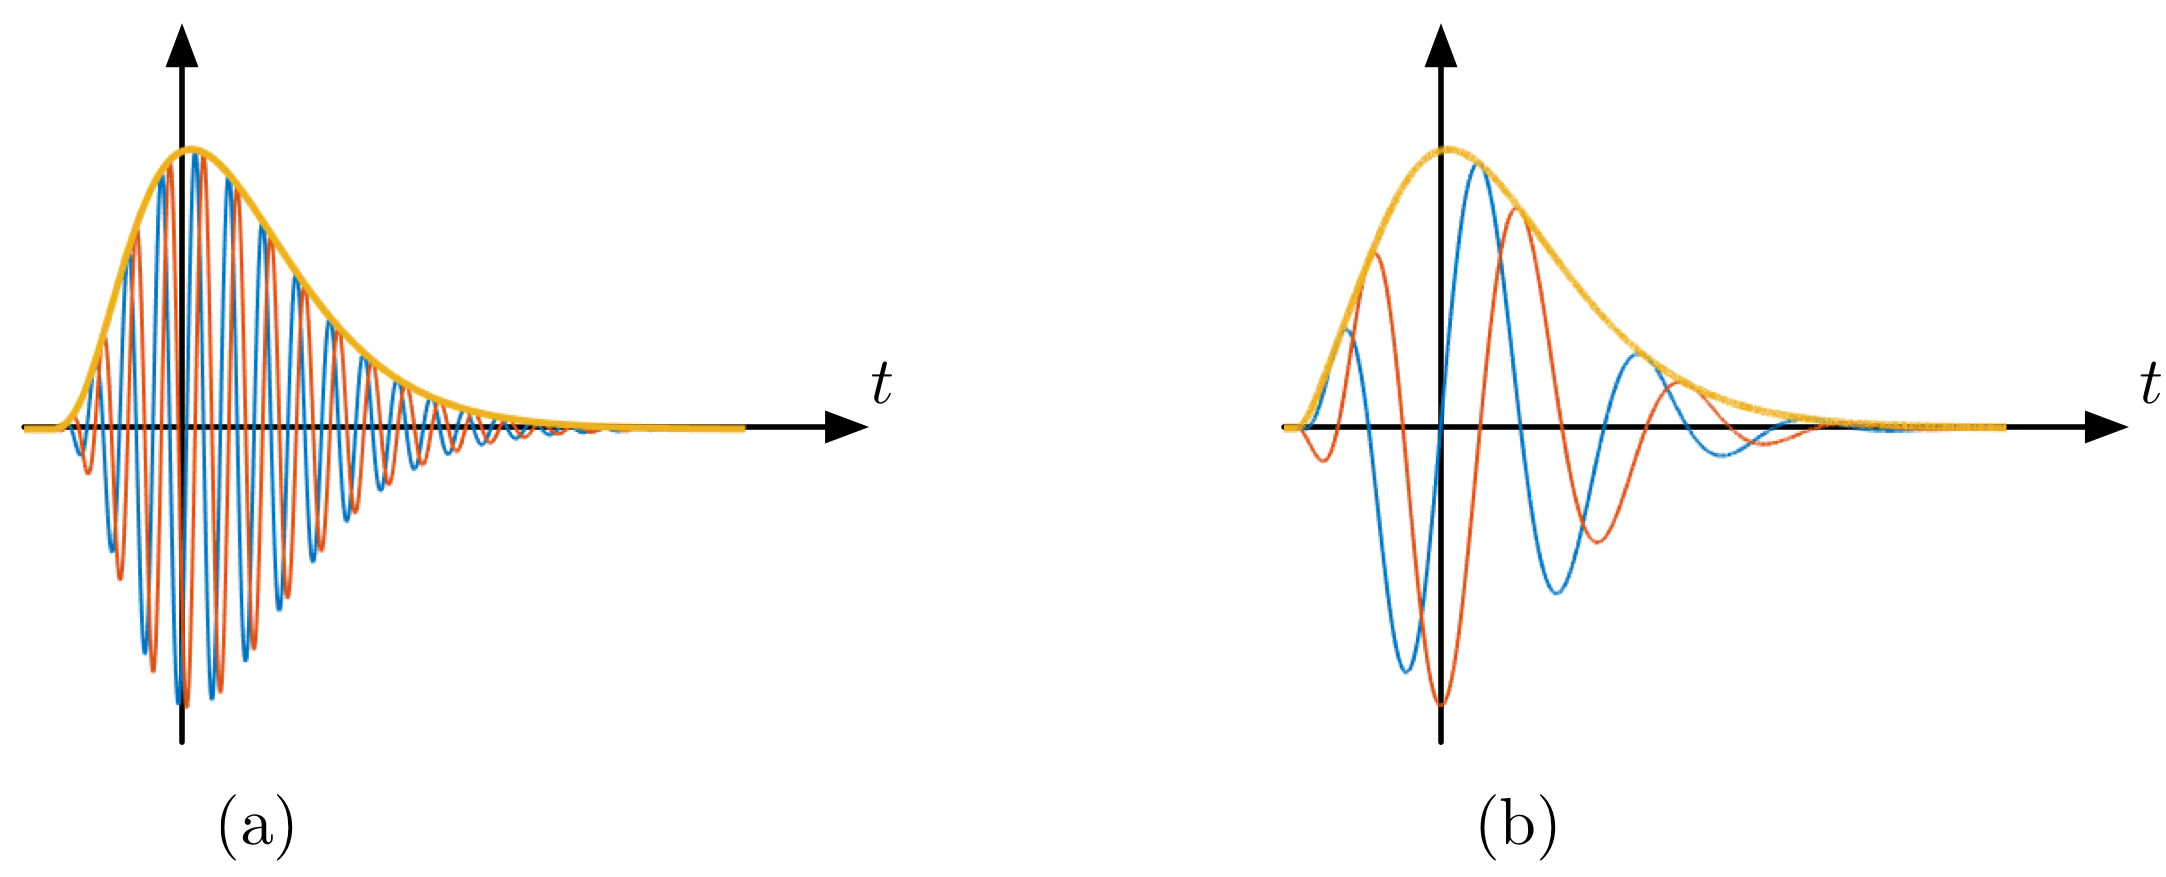
\includegraphics[width=\columnwidth]{figures/gammatones}
\caption{
\label{fig:gammatones}
Gammatone wavelets $\psi(t)$ in the time domain with quality factors (a) $Q = 4$ and (b) $Q = 1$.
Oscillations (red, blue) are the real and imaginary parts. The envelope (yellow) is the complex modulus.}
\end{center}
\end{figure}
Wavelets
$\boldsymbol{\psi_{\gamma_1}}(t)$ and $\boldsymbol{\psi_{\gamma_2}}(t)$ are designed as fourth-order Gammatone
wavelets with one vanishing moment \cite{Venkitaraman2014}, and are shown in Figure \ref{fig:gammatones}.
In the context of auditory scene analysis, the asymmetric envelopes of Gammatone wavelets are more biologically plausible than the symmetric, Gaussian envelopes of the more widely used Morlet wavelets.
Indeed, it allows to reproduce two important psychoacoustic effects in the mammalian cochlea: the asymmetry of temporal masking and the asymmetry of spectral masking  \cite{Fastl2007}.
The asymmetry of temporal masking is the fact that a masking noise has to be louder if placed after the onset of a stimulus rather than before.
Likewise, because critical bands are skewed towards higher frequencies, a masker tone has to be louder if it is above the stimulus in frequency rather than below.

It should also be noted that Gammatone wavelets follow the typical amplitude profile of natural sounds, beginning with a relatively sharp attack and ending with a slower decay.
As such, they are similar to filters discovered automatically by unsupervised encoding of natural sounds \cite{Smith2006}.
This suggests that, despite being hand-crafted and not learned, Gammatone wavelets provide a sparser time-frequency representation of acoustic scenes compared to other variants.

\section{Feature design}
\label{sec:design}

Before constructing models for similarity estimation, it is beneficial to process scattering coefficients to improve invariance, normality, and generalization power.
In this section, we review two transformations which achieve these properties: logarithmic compression and standardisation.

\subsection{Logarithmic compression}
\label{sec:logcomp}

Many algorithms in pattern recognition, including nearest neighbor classifiers and SVMs, tend to work best when all features follow a standard normal distribution across all training instances \cite{Hsu2003}.
Yet the distribution of the scattering coefficients is skewed towards larger values. We can reduce this skewness by applying a pointwise concave transformation to all coefficients. In particular, we find that the logarithm performs particularly well in this respect.
Figure \ref{fig:histograms} shows the distribution of an arbitrarily chosen scattering coefficient over the DCASE 2013 dataset, before and after logarithmic compression.

\begin{figure}
\begin{center}
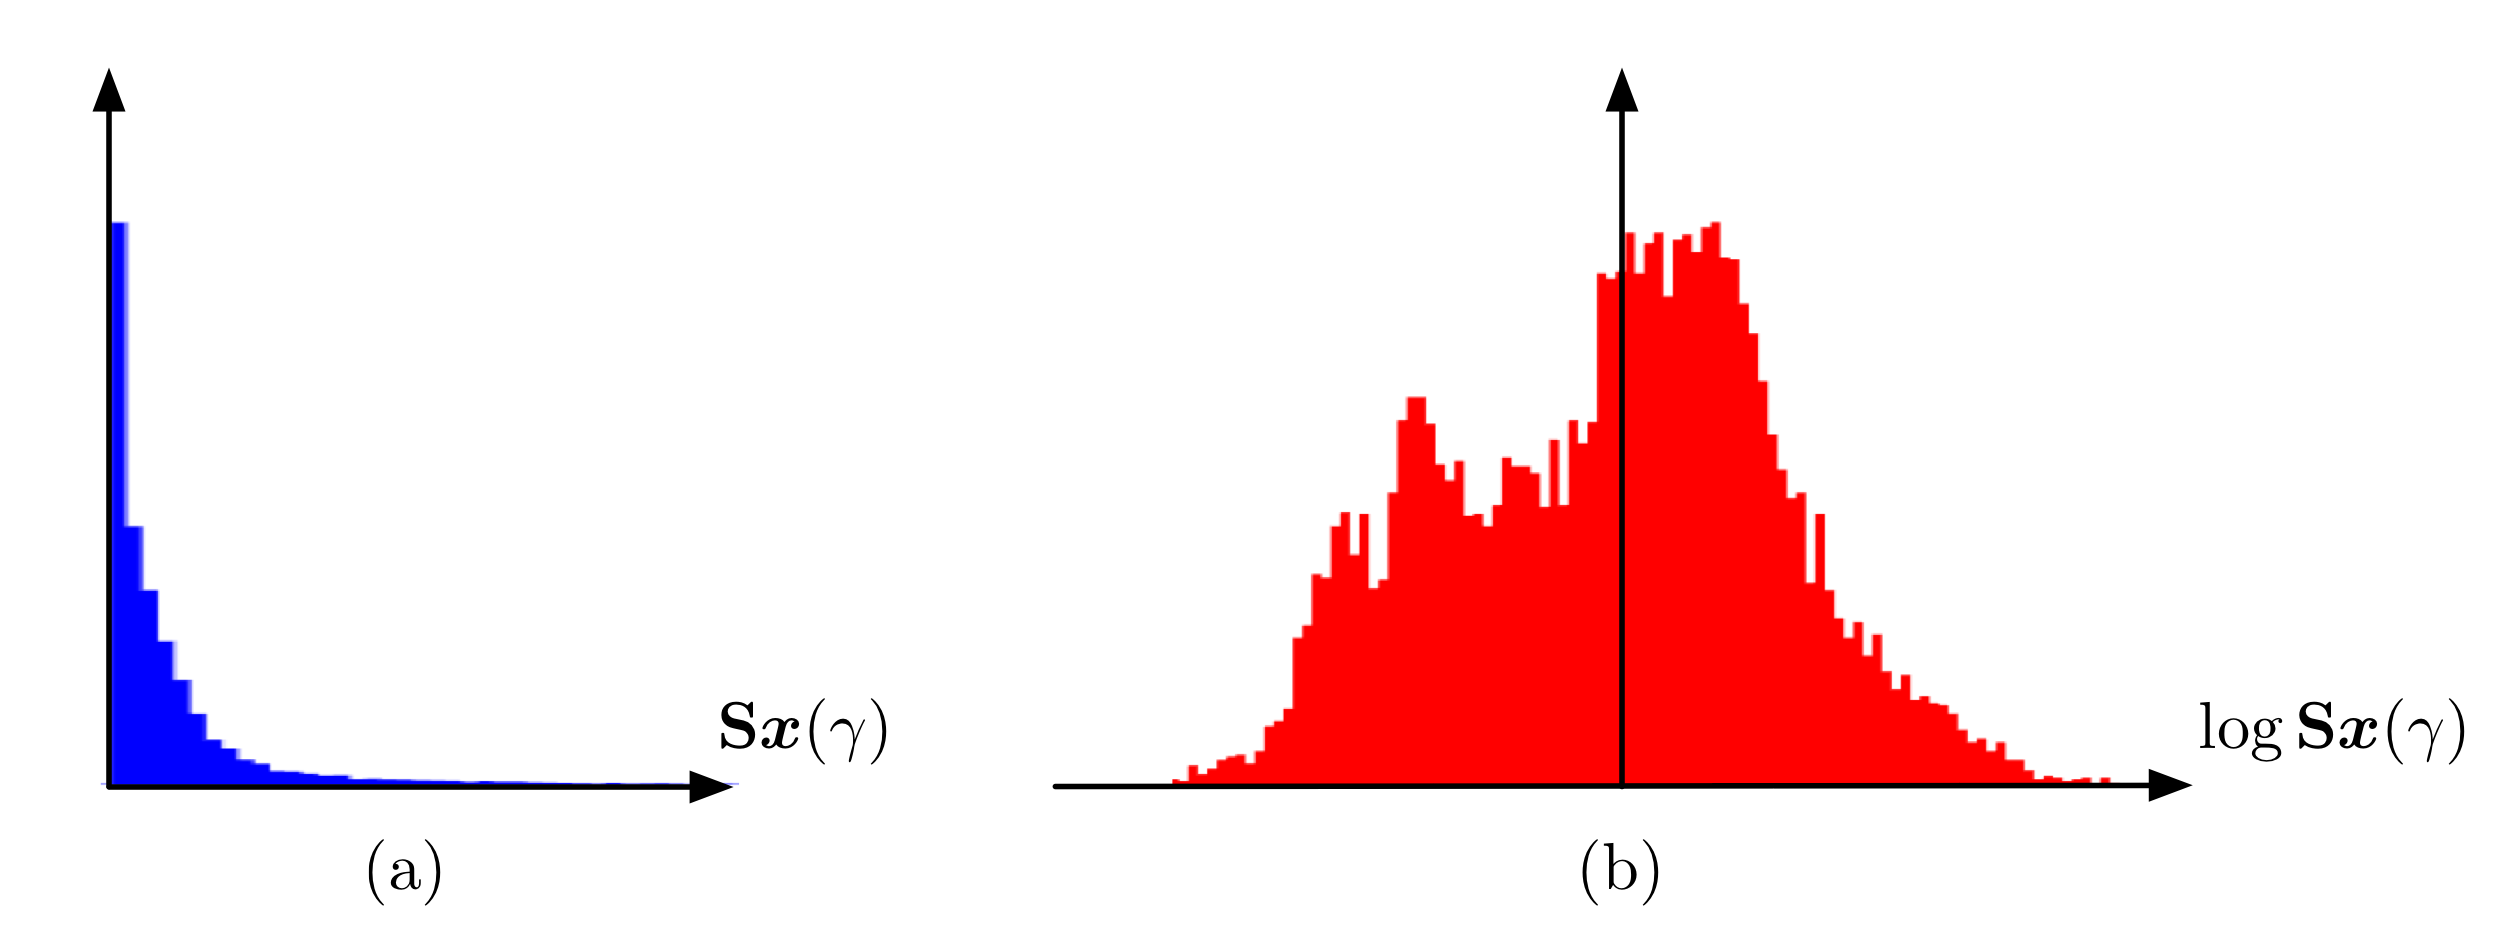
\includegraphics[width=\columnwidth]{figures/compression}
\caption{
\label{fig:histograms}
Histogram of values taken by the first-order scattering coefficient $\mathbf{S}\boldsymbol{x}(\gamma)$, corresponding to a center acoustic frequency of $302\,\mathrm{Hz}$,
(a) before and (b) after logarithmic compression.}
\label{fig:compression}
\end{center}
\end{figure}

Taking the logarithm of a magnitude spectrum is ubiquitous in audio signal processing.
Indeed, it is corroborated by the Weber-Fechner law in psychoacoustics, which states that the sensation of loudness is roughly proportional to the logarithm of the acoustic pressure.
We must also recall that the measured amplitude of sound sources often decays polynomially with the distance to the microphone--a source of spurious variability in scene classification.
Logarithmic compression linearizes this dependency, facilitating the construction of powerful invariants at the classifier stage.

\subsection{Standardisation}
\label{sec:stand}

Let $\mathbf{S}\boldsymbol{x}(\gamma,n)$ be a dataset, where $\gamma$ and $n$ denote feature and sample indices, respectively.
Many algorithms operate better on features which have zero mean and unit variance to avoid mismatch in numeric ranges \cite{Hsu2003}.
To standardise $\mathbf{S}\boldsymbol{x}(\gamma,n)$, we subtract the sample mean vector $\mu[\mathbf{S}\boldsymbol{x}(\gamma)]$ from $\mathbf{S}\boldsymbol{x}(\gamma,n)$ and divide the result by the sample standard deviation vector $\sigma[\mathbf{S}\boldsymbol{x}] (\gamma)$.
The vectors $\mu[\mathbf{S}\boldsymbol{x}(\gamma)]$ and $\sigma[\mathbf{S}\boldsymbol{x}](\gamma)$ are estimated from the entire dataset.

\section{Acoustic scene similarity retrieval}
\label{sec:object}

%As part of the aforementioned research areas and applications, the emerging field of \emph{Acoustic Scene Analysis} (also called \emph{Sound Scene Analysis}) \cite{Stowell15} aims to develop approaches and systems for the automatic analysis of environmental sounds and soundscapes (originating both from urban or nature environments). While research methodologies in related fields such as Automatic Speech Recognition (ASR) \cite{Rabiner93} and Music Information Retrieval (MIR) \cite{Muller07} are now well established, research addressing Acoustic Scene Analysis remains relatively young.

%From a data processing point of view, a holistic scheme, such as the bag-of-frame approach \cite{aucouturier2007bag}, has a simplicity, but clearly face poor performance on realistic conditions \cite{lagrange:hal-01082501}.

As discussed in Section \ref{sec:soa}, results in sound perception suggest the appropriateness of source-driven representations of auditory scenes for predicting high-level properties. While this can be addressed in the supervised case using late integration of discriminative classifiers \cite{Anden2014}, this is not directly feasible in the unsupervised case. As the detection of events is still an open problem \cite{7100934}, we consider in this paper a generic quantization scheme in order to identify and represent time intervals of the scene that are coherent, thus likely to be dominated by a given source of interest.

Given a set of $d$-dimensional feature vectors $X_u = \{x_1^u, \ldots, x_L^u\}$, extracted from the scene $s_u$, where $u=\lbrace 1,2,\ldots,U\rbrace$, we would like to partition $X_u$ into a set $C_u = \{c^u_1, \ldots, c^u_M\}$ of $M$ clusters. The partitioning is done by minimizing squared error between the empirical mean, or centroid, of each cluster and the vectors belonging to it. This is known as $k$-means clustering \cite{lloyd} and has found widespread use for a variety of applications.
Each scene $s_u$ is then described by a set of clusters $C_u$. One should note that this quantization approach differs from unsupervised learning schemes such as the ones studied in \cite{bisot2016acoustic}, where the scene features are projected in a dictionary learned from the entire dataset. Here, with the aim of better balancing the influence of salient sound events and texture-like sounds on the final decision, the similarity between two scenes is computed based on the similarity of their centroids.

The similarity between the scene centroids $\mu_m^u$ over the entire dataset, is computed using a radial basis function (RBF) kernel $K$ combined with a local scaling method \cite{selfTuneManor2004}:
\begin{equation}
\label{eq:kc}
K_{mn}^{uv} = \exp\left( - \dfrac{\Vert \mu_m^u - \mu_n^v \Vert^2}{\Vert \mu_m^u - \mu_{m,q}^u \Vert \Vert \mu_n^v - \mu_{n,q}^v \Vert} \right).
\end{equation}
Here, $\mu_{m,q}^u$ and $\mu_{n,q}^v$ are the $q^{\textrm{th}}$ nearest neighbors to the centroids $\mu_m^u$ and $\mu_n^v$, respectively, and $\Vert \cdot \Vert$ denotes the Euclidean norm.

To compute the similarity between two scenes, we consider several centroid-based similarity metrics:
\begin{itemize}
\item Relevance-based Quantization closest similarity (\emph{RbQ-c}): the similarity between two scenes $s_u$ and $s_v$ is equal to the largest similarity between their centroids, that is
\begin{equation}
	\max_{m,n} K_{mn}^{uv},
\end{equation}
\item Relevance-based Quantization average similarity  (\emph{RbQ-a}): the similarity between two scenes $s_u$ and $s_v$ is equal to the average of their centroid similarities, that is
\begin{equation}
	\frac{1}{M^2} \sum_{m,n} K_{mn}^{uv}
\end{equation}
and,
\item Relevance-based Quantization weighted similarity  (\emph{RbQ-w}): the similarity between two scenes is computed using a variant of the earth mover's distance applied to the set of centroids each weighted by the number of frames assigned to its cluster.
\end{itemize}

For \emph{RbQ-w}, each scene is represented by a signature
$$
p_u = \lbrace(\mu_1^u,w_1^u),(\mu_2^u,w_2^u),\ldots,(\mu_M^u,w_M^u)\rbrace,
$$
where each of the $M$ centroids $\mu_1^u, \ldots, \mu_M^u$ are paired with corresponding weights $w_1^u, \ldots, w_M^u$. The weight $w_m^u$ for the $m$th centroid $\mu_m^u$ is the number of frames belonging to a particular cluster. The similarity between scenes is then given by a cross-bin histogram distance known as the non-normalized earth mover's distance ($\widehat{\EMD}$) introduced by \cite{pele2008linear}. The $\widehat{\EMD}$ computes the distance between two histograms by finding the minimal cost for transforming one histogram into the other, where cost is measured by the number of transported histogram counts multiplied with the ``ground distance'' between the histogram bins. %In our case, the histogram counts are the clusters weights $w_m^u$ defined over the bins formed by the centroids $\mu_m^u$, so the ground distance is the centroid distance. \ml{From what we have below, the distance is not actually the distance between centroids, though. It's given by the kernel $K_{mn}^{uv}$.}

%\ml{Do we need the details that follow? Is it not enough to refer to \cite{pele2009fast}?}
%To compute the $\widehat{\EMD}$, we use the implementation proposed in \cite{pele2009fast}. Given two signatures $p_u$ and $p_v$, the $\widehat{\EMD}$ is computed by solving the following linear program:
% \begin{equation}
% \begin{split}
% \widehat{\EMD}(p_u,p_v) &=\left( \min\limits_{\lbrace f_{nm}\rbrace} \sum\limits_{n,m} f_{nm}D_{nm}^{uv} \right) \\
% &+ \left|\sum\limits_{n} w_n^u - \sum\limits_{m} w_m^v  \right| \max\limits_{n,m}\lbrace  D_{nm}^{uv}\rbrace.
% \end{split}
% \end{equation}
%
% \begin{equation*}
% \mathrm{s.t.} \quad f_{nm}\geq0 \quad \sum\limits_{m} f_{nm} \leq w_n^u \quad \sum\limits_{n} f_{nm} \leq w_m^v
% \end{equation*}
%
% \begin{equation*}
% \sum\limits_{n,m}f_{nm} = \min\left( \sum\limits_{n} w_n^u ,\sum\limits_{m} w_m^v \right)
% \end{equation*}
% %\ja{Can we provide some interpretation for the different terms and constraints here?}
% where $\lbrace f_{nm} \rbrace$ is the flow between the cluster weights $w_n^u$ and $w_m^v$, that is, the amount transported from the $n^{\textrm{th}}$ bin to ``supply the demand'' of the $m^\textrm{th}$ bin. We denote by $D^{uv}$ the ground distance, a matrix containing the pairwise distances between the centroids sets $\mu^u$ and $\mu^v$ which is computed from $K$:
% \begin{equation*}
% D_{mn}^{uv}=1-K_{mn}^{uv}.
% \end{equation*}
% \ml{Note that this is not actually a distance.}

% To get the final similarity measure between the scenes $s_u$ and $s_v$, an extended Gaussian kernel $K^s$ is computed: %\cite{chapelle1999support,jing2003support}
% \begin{equation}
% \label{eq:ks}
% K_{uv}^s = \exp\left( - \dfrac{\widehat{\EMD}(p_u,p_v)}{A} \right) \\
% \end{equation}
% with $A$ a scaling parameter, set to the mean value of the $\widehat{\EMD}$ between all the scenes. The resulting kernel $K^s$ is known as an $\EMD$ kernel, and it should be noted that there is no guarantee that this kernel is positive definite. \ml{Is this kernel used anywhere? For similarity, do we not just use the EMD distance directly?}

\section{Experiments}
\label{sec:experiments}

To evaluate the representations introduced in the previous section, we apply it to the acoustic scene similarity retrieval task on the DCASE 2013 dataset.
Results demonstrate the improved performance of the relevance-based quantization of scattering coefficients compared to baseline methods using summary statistics of MFCCs.
The implementations of the presented methods and the experimental protocol are available online.\footnote{\url{https://github.com/mathieulagrange/paperRelevanceBasedSimilarity}} % \ja{What is ``the one''?}

% , and $\alpha$ is a parameter which trades off between \ja{?}

\subsection{Dataset}

%For most of the experiments reported in this paper, we will consider the DCASE2013 dataset \cite{giannoulis2013database, 7100934}. Larger datasets exists: the
%Rouen dataset \cite{rakotomamonjy2015histogram} and the public part of the DCASE2016 challenge.%
The experiments in this paper are carried out on the DCASE 2013 \cite{7100934} dataset.
This dataset consists of two parts, namely a public and a private subset, each made up of $100$ acoustic scene recordings, sampled at $44100\,\mathrm{Hz}$ and $30$ seconds in duration. The dataset is evenly divided into $10$ acoustic scence classes. The recordings were made by three different recordists at a wide variety of locations in the Greater London area over a period of several months. No
systematic variations in the recordings covaried with scene
type: all recordings were made under moderate weather conditions, at varying times of day and week, and each recordist recorded each scene type. As a result, the DCASE 2013 dataset enjoys significant intra-class diversity while remaining of manageable size, making it suitable for extensive evaluation of algorithmic design choices \cite{lagrange:hal-01082501}.
%In addition, it is still a challenging dataset, with a state-of-the-art system based using handcrafted features as input to SVMs achieving $76\%$ \cite{roma2013} (winner of the DCASE2013 challenge), while recent approaches based on label tree embedding achieve between $84\%$ and $87\%$ on DCASE 2013 depending on the prior knowledge used during training \cite{phan2016label}.

%Recent advances using hierarchical classifier architectures obtain between $84\%$ and $87\%$ on DCASE2013 depending on the prior knowledge used during training \cite{phan2016label}. On the Rouen dataset, the state-of-the-art is currently $95\%$ \cite{bisot2016acoustic}.
%, but here we conduct our experiments on the public part of the dataset. \ja{Any more information on this dataset?}

%In this paper, we are interested in evaluating different algorithmic designs leading to different scene models, we therefore resort to straightforward ranking performance measures for the ASSR task. \ja{It's not clear to me how the first part implies the second part here} Similarly, we have picked SVMs as our classifier for the ASC task, since these are a standard tool in the community and allows for us to focus our analysis on the earlier processing stages. Moreover, since MFCCs are well-established features which perform well for these task, we shall include them baseline features in all experiments described in this paper.

\subsection{Feature design}

Experiments are carried out using scattering coefficients as well as baseline mel-frequency cepstral coefficients (MFCCs) as features. For the scattering transform, each $30$-second scene is described by $128$ vectors computed with half-overlapping windows $\boldsymbol{\phi}(t)$ of duration $T=372\,\mathrm{ms}$, for a total of $24\,\mathrm{s}$. In this case, $3$ seconds are discarded at the beginning and end of the scene to avoid boundary artifacts. Experiments are conducted with and without logarithmic compression (see Section \ref{sec:logcomp}).

MFCCs are computed for windows of $50\,\mathrm{ms}$ and hops of $25\,\mathrm{ms}$ with full frequency range. The standard configuration of $39$ coefficients coupled with an average-energy measure performs best in preliminary tests, so we use this in the following. The coefficients are averaged using $250\,\mathrm{ms}$ long non-overlapping windows so that each window represents structures of similar scale to the scattering coefficients.

%. The MFCC vectors within each texture window are then averaged in time. As the \emph{ob} approaches involve a clustering step, we need to ensure that both MFCCs and scattering coefficients have a comparable number of vectors per recording. Thus, $t$ is set to $250\,\mathrm{ms}$, resulting in $120$ MFCCs texture windows per scene.

%\ja{We've tested the impact of the logarithm here, but not of the feature selection or standardization. Should we do this as well? For the feature selection, we did say earlier that we would test its impact.}

%Having validated the underlying assumptions for the cluster-based auditory scene representation, we evaluate its performance for the task of acoustic scene similarity retrieval. \ml{What does this mean?}

\subsection{Algorithm}

The evaluation is performed on the private part of the DCASE 2013 dataset. The metric used is the precision at rank $k$ ($p@k$), which is computed by taking a query item and counting the number of items of the same class within the $k$ closest neighbors, and then averaging over all query items. These closest neighbors are determined by a particular distance, which is one of \emph{RbQ-c}, \emph{RbQ-a}, or \emph{RbQ-w}. \vl{Avoid passive voice.}

The metric $p@k$ is computed for $k=\lbrace 1,\ldots,9\rbrace$, since each class only has $10$ items. Note that a $p@1$ is equivalent to the classification accuracy obtained by the classifier which chooses the label of the closest neighbor for a given item. The \emph{RbQ} approaches are compared to commonly used early integration approach \emph{early}, which consists in averaging over time the feature set of each scene, resulting in one feature vector per scene. The parameters of the BOF approach are the one used in \cite{aucouturier2007bag}, \textit{i.e.} 10 Gaussians per scene estimated using the Expectation Maximization (EM) algorithm. Gaussian models are compared using Monte-Carlo sampling approximation. In order to ensure convergence of the EM algorithm when considering the scattering features as input, the dimension of the feature vector is reduced from 1367 to 30 by projecting the features over the 30 principal components computed over the whole dataset. \vl{Too much passive voice, too many instances of "use", "used".}

The scaling parameter $q$ of the RBF kernels (see Eq. \ref{eq:kc}) is set to $10\%$ of the number of data points to cluster.%, being the number of scenes for \emph{early} and the number of clusters for RbQ approaches. \ml{What does this mean?}
The clustering for the \emph{RbQ} approaches is done using plain $k$-means with random initialization and $200$ replicates. For each method, the numbers of clusters is set to $8$.

%\ja{I'm not sure what this means. Do we fix $m$ and $N$ here for all experiments or do we optimize them over the test data each time? If so, this will bias the results, no?}

\section{Results \label{sec:results}}

%The results on acoustic scene classification illustrate the superior performance of the log-scattering transform coupled with late integration, confirming the ideas motivating the construction of our cluster-based auditory scene representation. Using this representation for auditory scene similarity retrieval, we obtain results that improve significantly over traditional BOF and summary approaches, both with log-scattering and MFCCs features.


This section presents evaluation results for the acoustic scene similarity retrieval task. The $p@k$ for different settings are shown in Figure \ref{fig:ASS_1}, illustrating the effect of the different similarity metrics. This allows us to also evaluate the recall capabilities of the system under evaluation.

\subsubsection*{Baselines}

As can be seen on Figure \ref{fig:ASS_-1}, the BOF approach behaves similarly to the early approach when considering MFCCs as features. Its performance decreases compared to the early approach when considering the scattering features. Extensive analysis of those results is out of the scope of this paper, but we can assume that this decrease is to to the dimensionality reduction operated on the scattering features before GMM training in order to ensure the convergence of the EM algorithm.

The early approach being simpler in terms of implementation and runtime complexity, this method is retained as baseline for the remaining.

\begin{figure}[t]
\begin{center}

\includegraphics[width=\columnwidth]{figures/baselines}
\caption{Acoustic scene similarity retrieval in the DCASE 2013 private dataset: precisions at rank $k$ ($p@k$) obtained for scattering with or without logarithmic compression, as a function of the rank $k$.
\vl{The x-axis label is wrong. precision should be replaced by "rank $k$". The y-axis should be "precision ($p@k$)". It would be good to have the y-axis range from $0\%$ to $100\%$.
The lines should be thicker and follow a color palette of complementary colors (blue vs. orange). The legends should not be abbreviated: scatT -> scattering, mfcc -> MFCC. }}
\label{fig:ASS_-1}
\end{center}
\end{figure}

\subsubsection*{Logarithmic compression}

As can be seen on Figure \ref{fig:ASS_0}, the logarithmic compression is beneficial for precision performance irrespective of the similarity considered. The gain is more pronounced when considering alternative similarities.

\begin{figure}[t]
\begin{center}
\includegraphics[width=\columnwidth]{figures/log}
\caption{Acoustic scene similarity retrieval in the DCASE 2013 private dataset: precisions at rank $k$ ($p@k$) obtained for scattering with or without logarithmic compression, as a function of the rank $k$.}
\label{fig:ASS_0}
\end{center}
\end{figure}

\subsubsection*{MFCC \vs scattering transform}

Irrespective of the rank $k$ considered, best result is achieved for the scattering transform with logarithmic compression using the \emph{RbQ-c} approach. Overall, log-compressed scattering coefficients systematically outperform MFCCs. This is to be expected since the scattering coefficients capture larger-scale modulations, as opposed to MFCCs which only describe the short-time spectral envelope.

\subsubsection*{Relevance-based quantization \vs early integration}

For the scattering transform, both \emph{RbQ-c} and \emph{RbQ-w} outperform \emph{early}, thus confirming the benefits of using an relevance-based quantization (\emph{RbQ}) to improve the similarity measures between the scenes. However, it is worth noticing that \emph{RbQ-a} performs worse or comparably to \emph{early}, showing that the discriminant information is destroyed by averaging the contributions from all centroids. This result is in line with the findings of \cite{lagrange:hal-01082501}. To take advantage of such a representation, we need to select certain representative centroids when comparing quantized objects. Furthermore, it appears that \emph{RbQ-c} is better able to characterize the classes compared to \emph{RbQ-w}. This last observation suggests that weighting a centroid according to the number of frames it contains may prove to be a limited solution. Indeed, nothing a priori indicates that the discriminant information between two scenes lays within the majority of their frames. On the contrary, two similar environments may share a lot of similar sound sources with only a few sources discriminating between them. \ml{This is a bit of a stretch, since it may just be that we used the wrong distance to take the weighting into account. Perhaps the non-normalized EMD is not appropriate here?}

\ja{needs to be discussed}

Considering $p@5$ as our metric (as in \cite{aucouturier2007bag} and \cite{lagrange:hal-01082501}), the use of the log-scattering transform instead of MFCCs increases the performance from $0.31$ to $0.49$ and the use of the relevance-based quantization approach using the closest similarity (\emph{RbQ-c}) further improves the performance to $0.54$ for a global increase of $0.23$. \vl{Too many instances of ``use'', ``use'', ``using''. It is worth reminding what the baselines are.}

%The same observations are made for the MFCCs for $k\leq5$. However for a rank $k$ greater than $5$, all the \emph{RbQ} approaches perform equivalently. As such, one can conclude that the use of MFCCs allows us to retrieve closely related scenes, but their lack of discriminative capabilities making the cluster selection/weighting step useless for not so closely related scenes of the same class.

%This may be due to the fact that, at some point, the MFCCs fail to dissociate the discriminative events of a scene from the non-informative ones, thus making the cluster selection/weighting step useless. \ja{What is the ``at some point'' referring to? In other words, why do we expect this to happen for larger $k$ but not smaller?}

%However for a rank $k$ greater than $5$, there is no clear evidence that \emph{ob-c} and \emph{ob-w} approaches improve the results compared to \emph{early}. The latter even outperforms \emph{ob-a} for $k\geq5$. From this it appears that, although the \emph{ob} approaches are able to better retrieve the similarities between close scenes compared to \emph{early}, they are of no help when considering distant scenes of the same class. This may be due to the fact that, at some point, the MFCCs fail to dissociate the discriminative events of a scene from the non-informative ones, thus making a centroid-based description useless, or even counterproductive when the centroids are not weighted/selected.

\begin{figure}[t]
\begin{center}
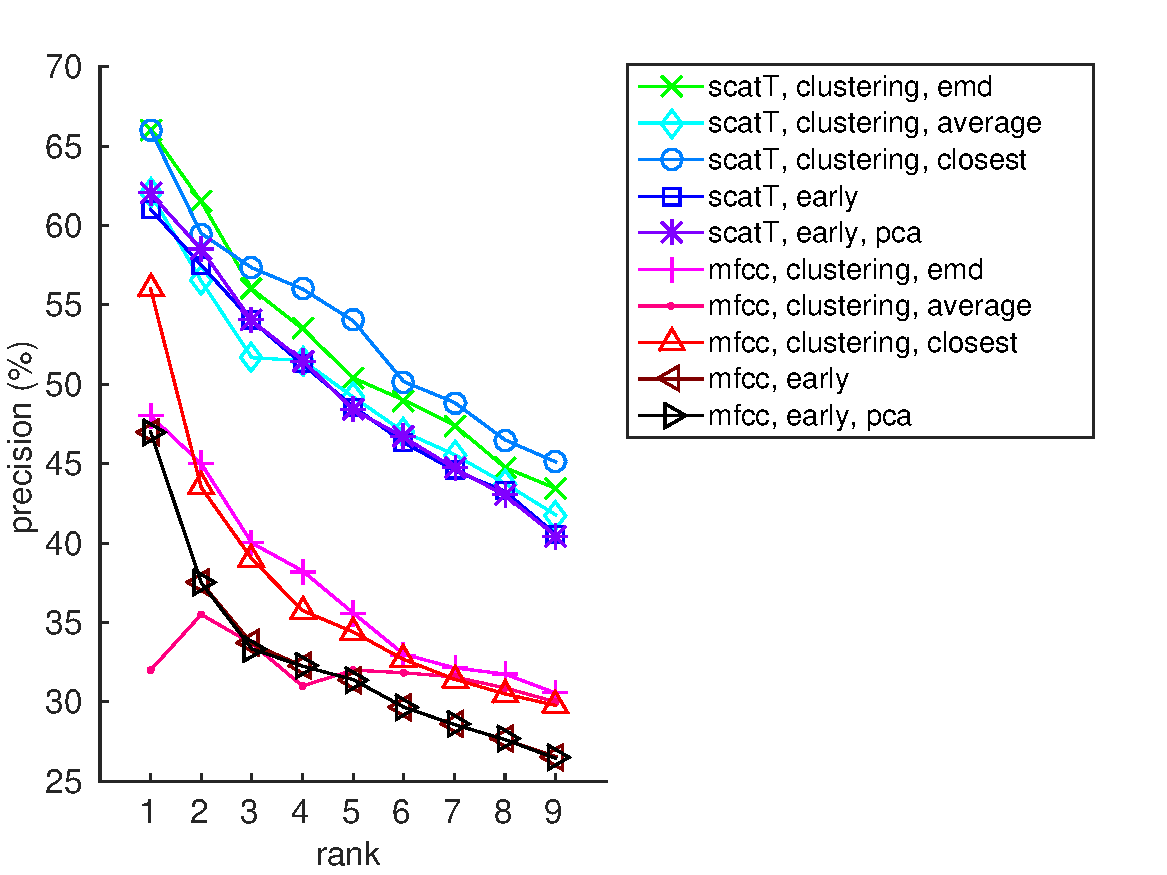
\includegraphics[width=\columnwidth]{figures/overall}
\caption{Acoustic scene similarity retrieval in the DCASE 2013 private dataset: precisions at rank $k$ ($p@k$) obtained for MFCCs and scattering with logarithmic compression, as a function of the rank $k$.}
\label{fig:ASS_1}
\end{center}
\end{figure}

\section{Conclusion}

This paper presents a new approach for modeling acoustic scenes which utilizes scattering transforms at small scales and a cluster-based representation at large scales. Compared to traditional models based on BOF and summary statistics, this representation allows for the characterization of distinct sound events superimposed on a stationary texture, a concept which has strong grounding in the cognitive psychology literature. In order to extend the selectivity potential of late integration using SVMs to the unsupervised case, we develop the cluster-based model and validate it using experiments on acoustic scene similarity retrieval. For this task, we show significant improvements over the traditional BOF and summary statistics models based on both standard MFCCs and scattering features.
These outcomes shall be studied further in future work by considering larger databases and emerging tasks in computational bioacoustics \cite{wimmer2013sampling}.
\vl{The verb utilize should be avoided.}

%\bibliographystyle{spmpsci}
%\bibliography{biblio}
\printbibliography

% \begin{IEEEbiography}[{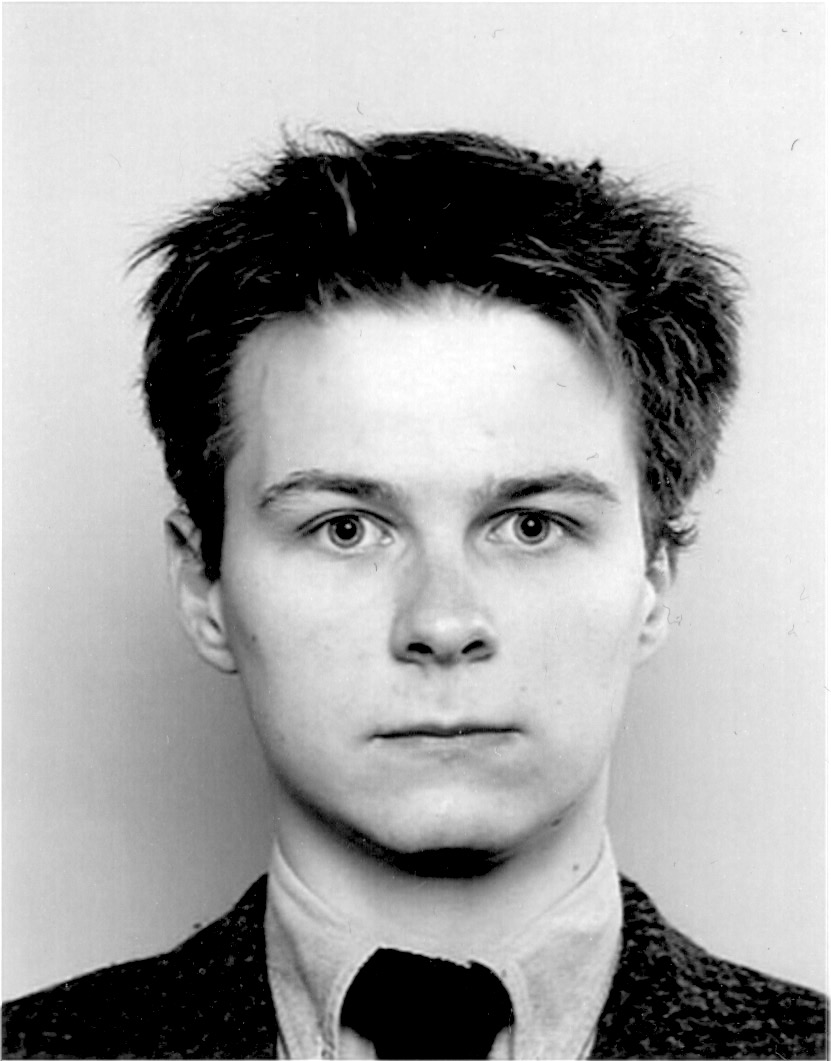
\includegraphics[width=1in,height=1.25in,clip,keepaspectratio]{figures/lostanlen}}]{Vincent Lostanlen} was born in 1992. He received an engineering degree from TELECOM ParisTech in 2013 and his M.S. degree in acoustics, signal processing, and musical informatics (ATIAM) from the Universit\'{e} Pierre et Marie Curie (UPMC) and the Ircam in Paris, France, in 2013. Since 2013, he is a Ph.D. student at \'{E}cole normale sup\'{e}rieure in Paris, working under the supervision of St\'{e}phane Mallat. His research focuses on defining convolutional operators in the time-frequency domain with applications in audio classification.
% \end{IEEEbiography}
%
% \begin{IEEEbiography}[{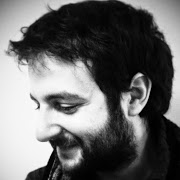
\includegraphics[width=1in,height=1.25in,clip,keepaspectratio]{figures/lafay}}]{Gr\'egoire Lafay} was born in 1990. He received the B.S. degree in Acoustic from the University Pierre and Marie Curie (UPMC), Paris, France, and the B.S. degree in Musicology from the Sorbonne University, Paris, France, in 2011. He received his M.S. degree in acoustics, signal processing, and musical informatics (ATIAM) from the UPMC and the Ircam in Paris, France, in 2013. Since 2013, he is a Ph.D. student at IRCCyN, Nantes, France. His research interests include acoustic scene similarity and classification as well as acoustic scene perception.
% \end{IEEEbiography}
%
%
% \begin{IEEEbiography}[{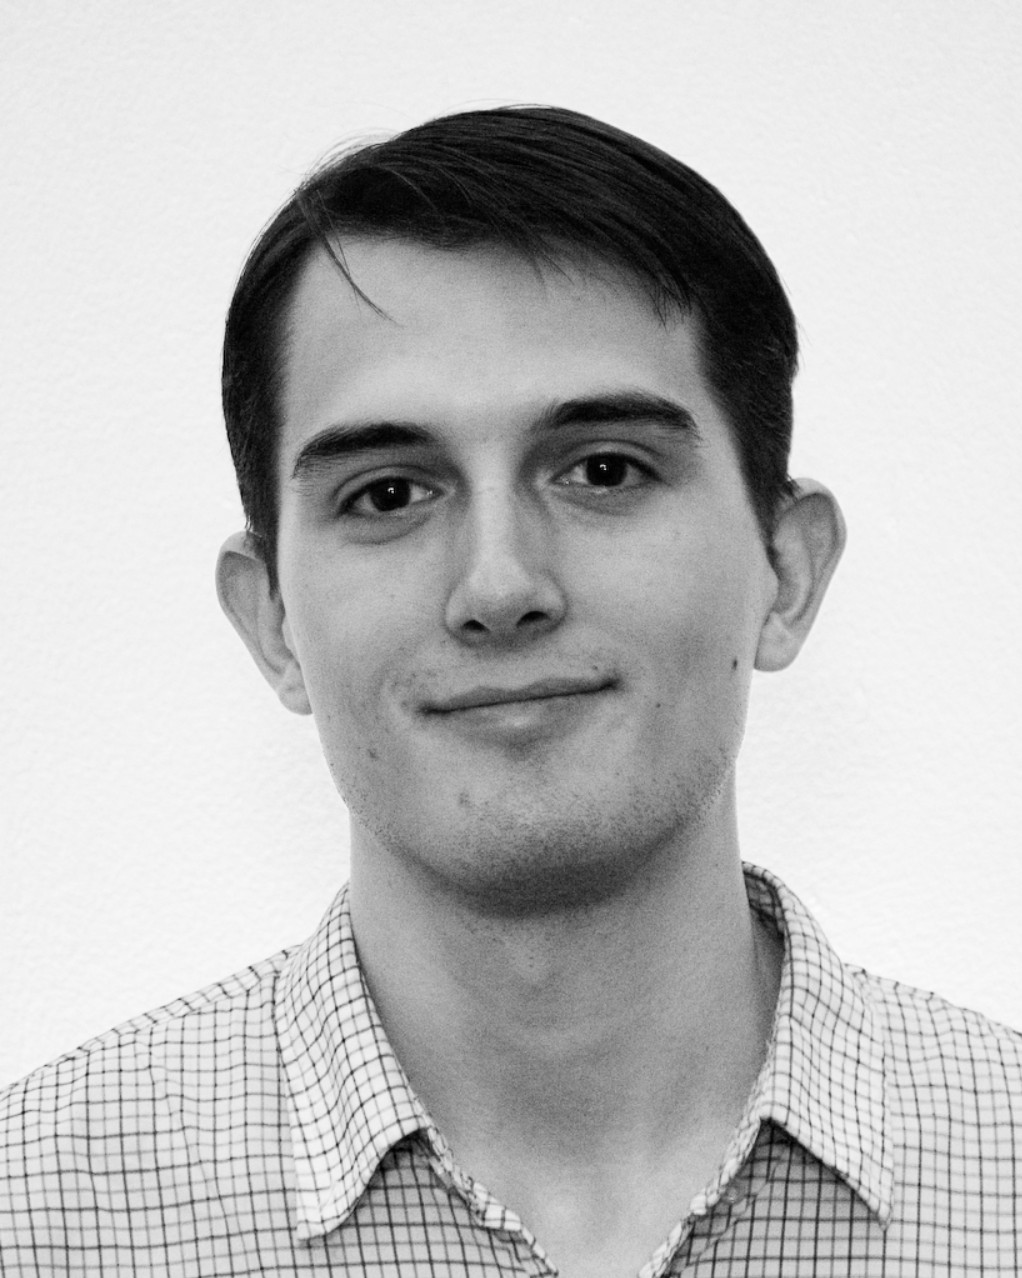
\includegraphics[width=1in,height=1.25in,clip,keepaspectratio]{figures/anden}}]{Joakim And\'en}
% received the M.Sc. degree in mathematics from the Universit\'e Pierre et Marie Curie, Paris, France, in 2010 and the Ph.D. degree in applied mathematics from Ecole Polytechnique, Palaiseau, France, in 2014. He is currently a postdoctoral researcher with the Program in Applied and Computational mathematics at Princeton University, Princeton, USA. His research interests include signal processing, machine learning, and statistical data analysis. He is a member of the IEEE.
%
% \end{IEEEbiography}
%
% \begin{IEEEbiography}[{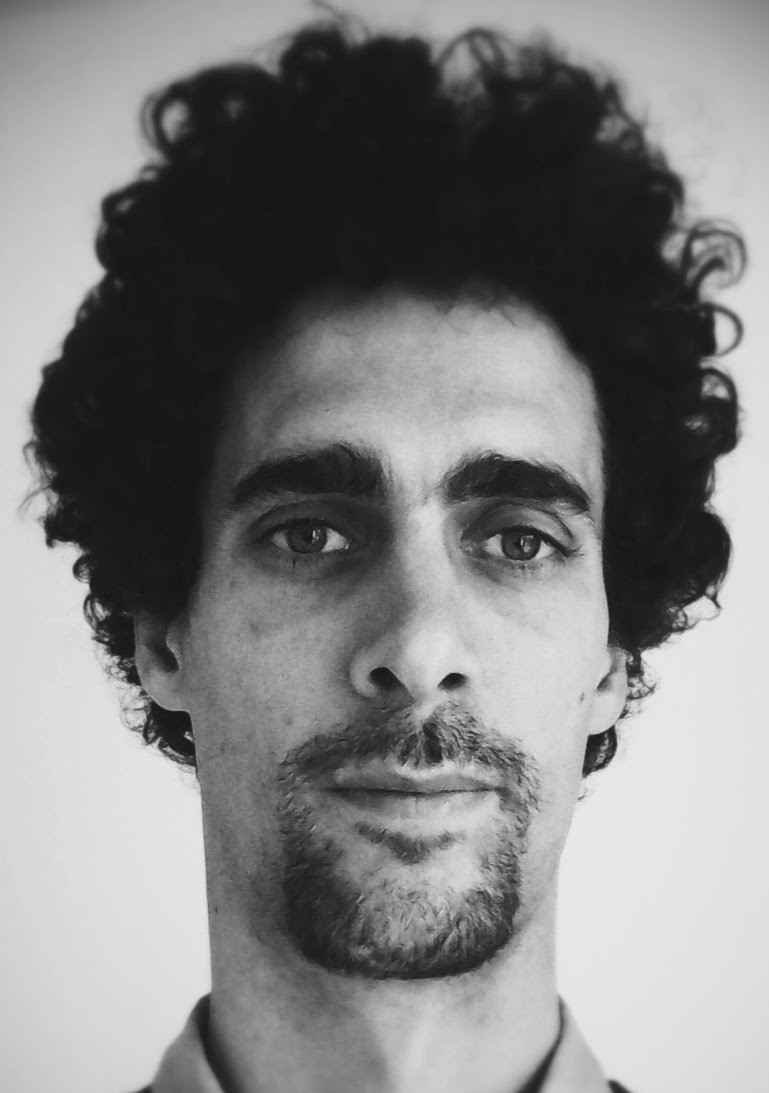
\includegraphics[width=1.25in,height=1.25in,clip,keepaspectratio]{figures/lagrange}}]{Mathieu Lagrange} is a CNRS research scientist at IRCCyN, a French laboratory dedicated to cybernetics. He obtained his Ph.D. in computer science at the University of Bordeaux in 2004, and visited several institutions in Canada (University of Victoria, McGill University) and in France (Orange Labs, TELECOM ParisTech, Ircam). His research focuses on machine listening algorithms applied to the analysis of musical and environmental audio.
% \end{IEEEbiography}

% biography section
%
% If you have an EPS/PDF photo (graphicx package needed) extra braces are
% needed around the contents of the optional argument to biography to prevent
% the LaTeX parser from getting confused when it sees the complicated
% \includegraphics command within an optional argument. (You could create
% your own custom macro containing the \includegraphics command to make things
% simpler here.)
%\begin{IEEEbiography}[{\includegraphics[width=1in,height=1.25in,clip,keepaspectratio]{mshell}}]{Michael Shell}
% or if you just want to reserve a space for a photo:

%\begin{IEEEbiography}{Mathieu Lagrange}
%Biography text here.
%\end{IEEEbiography}

% if you will not have a photo at all:
%\begin{IEEEbiographynophoto}{John Doe}
%Biography text here.
%\end{IEEEbiographynophoto}

% insert where needed to balance the two columns on the last page with
% biographies
%\newpage

%\begin{IEEEbiographynophoto}{Jane Doe}
%Biography text here.
%\end{IEEEbiographynophoto}

% You can push biographies down or up by placing
% a \vfill before or after them. The appropriate
% use of \vfill depends on what kind of text is
% on the last page and whether or not the columns
% are being equalized.

%\vfill

% Can be used to pull up biographies so that the bottom of the last one
% is flush with the other column.
%\enlargethispage{-5in}



% that's all folks
\end{document}
